%% LyX 2.1.2 created this file.  For more info, see http://www.lyx.org/.
%% Do not edit unless you really know what you are doing.
\documentclass[spanish]{beamer}
\usepackage[T1]{fontenc}
\usepackage[utf8]{inputenc}
\setcounter{secnumdepth}{3}
\setcounter{tocdepth}{3}
\usepackage{babel}
\addto\shorthandsspanish{\spanishdeactivate{~<>}}

\usepackage{textcomp}
\usepackage{graphicx}
\usepackage{setspace}
\PassOptionsToPackage{normalem}{ulem}
\usepackage{ulem}
\ifx\hypersetup\undefined
  \AtBeginDocument{%
    \hypersetup{unicode=true,
 bookmarks=false,
 breaklinks=false,pdfborder={0 0 0},backref=false,colorlinks=false,pdfpagemode=FullScreen}
  }
\else
  \hypersetup{unicode=true,
 bookmarks=false,
 breaklinks=false,pdfborder={0 0 0},backref=false,colorlinks=false,pdfpagemode=FullScreen}
\fi
\usepackage{breakurl}

\makeatletter

%%%%%%%%%%%%%%%%%%%%%%%%%%%%%% LyX specific LaTeX commands.
%% Because html converters don't know tabularnewline
\providecommand{\tabularnewline}{\\}

%%%%%%%%%%%%%%%%%%%%%%%%%%%%%% Textclass specific LaTeX commands.
 % this default might be overridden by plain title style
 \newcommand\makebeamertitle{\frame{\maketitle}}%
 % (ERT) argument for the TOC
 \AtBeginDocument{%
   \let\origtableofcontents=\tableofcontents
   \def\tableofcontents{\@ifnextchar[{\origtableofcontents}{\gobbletableofcontents}}
   \def\gobbletableofcontents#1{\origtableofcontents}
 }

%%%%%%%%%%%%%%%%%%%%%%%%%%%%%% User specified LaTeX commands.
\usetheme{Madrid}
%\usecolortheme{default}
\usecolortheme{seahorse}

 \date{}
\institute{}
\setbeamertemplate{footline}{}
%\usecolortheme[named=Mahogany]{structure}

\makeatother

\begin{document}

\title{Álgebra}


\subtitle{1º ESO}

\makebeamertitle

\begin{frame}{Índice}


\tableofcontents{}

\end{frame}

\section{Lenguaje algebraico}


\subsection{Expresiones Algebraicas}
\begin{frame}{Índice}


\begin{center}
\textbf{\Large{}EL LENGUAJE ALGEBRAICO}
\par\end{center}{\Large \par}

\end{frame}

\begin{frame}{¿Para qué usamos las letras?}

\begin{exampleblock}<1->{Ejemplo}
En el siguiente ejemplo aparecen letras que representan números
que todavía no conocemos. 

Investiga: 

Observa la siguiente suma:%
\begin{tabular}{cccc}
 & a & a & b\tabularnewline
+ & a & b & a\tabularnewline
\hline 
 & b & c & c\tabularnewline
\end{tabular}\hspace{1cm}
\includegraphics[width=0.3\paperwidth]{img/clase}

Si c es el número 3, ¿cuáles son los números a y b?\end{exampleblock}
\begin{alertblock}{Solución}\pause{}El 3 se puede descomponer como 0+3, 3+0 ó 1+2,
2+1. De todas las combinaciones, la única que cumple la suma sería
\textbf{a=1 y b=2}. \pause{}


Cuando no conocemos un número, podemos hacer referencia a él usando
\textbf{letras}. La parte de las matemáticas que utiliza expresiones
con letras y números se llama \textbf{Álgebra}.
\end{alertblock}
\end{frame}

\begin{frame}{El lenguaje algebraico}

\begin{block}<1->{Expresiones Algebraicas}Una \textbf{expresión algebraica} es una
combinación de letras, números y signos de operaciones.\pause{}

\begin{itemize}
\item $3x^{2}$, $x+2$, $2xy+5$ son expresiones algebraicas\pause{}
\item Observa como se expresan las siguientes operaciones:

\begin{itemize}
\item {\footnotesize{}$3\times x\times x$ es lo mismo que $3\cdot x\cdot x$,
y que $3\cdot x^{2}$. Por norma, se pone $3x^{2}$}{\footnotesize \par}
\item {\footnotesize{}$1\times x$ es lo mismo que $1x$. Por norma, se
pone solo $x$}{\footnotesize \par}
\end{itemize}
\end{itemize}
\end{block}

\pause{}
\begin{exampleblock}{Lenguaje Natural y Lenguaje Algebraico}


``Un número más 5'' podemos representarlo algebraicamente: $x+5$
\end{exampleblock}

\pause{}


\textbf{Ejercicios:} 


``siete menos un número cualquiera''\pause{}\dotfill{}${\color{red}7-x}$\pause{}


``ocho veces un número''\pause{}\dotfill{}${\color{red}8x}$\pause{}


``un número más otro''\pause{}\dotfill{}${\color{red}x+y}$

\end{frame}

\begin{frame}{Traducción de Enunciados}


\pause{}
\begin{block}{Ejemplo}
Juan y Oscar han pescado entre los dos 12 peces. Si representamos
mediante $x$ los peces que ha pescado Juan. ¿Cómo puedo expresar
en lenguaje algebraico los que ha pescado Oscar?

\begin{minipage}[c]{0.3\columnwidth}%
\begin{center}

\includegraphics{img/ninospescando}
\par\end{center}%
\end{minipage} \pause{}Oscar ha pescado\pause{}\rightarrowfill{}${\color{red}12-x}$
peces
\end{block}

\pause{}
\begin{block}{Ejemplo}
El precio por alquilar un coche es de 78€ por día más 0,12€ por km
recorrido. Si los alquilamos durante un día y representamos mediante
la letra $x$ los km recorridos, ¿cómo puedes expresar el importe
a pagar?

\begin{minipage}[c]{0.3\columnwidth}%
\begin{center}

\includegraphics[width=0.2\paperwidth]{img/aparcamiento}
\par\end{center}%
\end{minipage} \pause{}Hay que pagar\pause{}\rightarrowfill{}${\color{red}78+0,12x}$
euros
\end{block}
\end{frame}

\begin{frame}{Traducción de enunciados}


\pause{}
\begin{block}{Ejemplo}
Jugando a baloncesto, la puntuación de Joseba es el \textbf{doble}
que la de Miguel y éste tiene el \textbf{triple} que los obtenidos
por Indira \textbf{más uno}. Expresamos con $x$ la puntutación de
Indira:
\begin{columns}[c]


\column{3cm}



\includegraphics[width=0.2\paperwidth]{img/juego}


\column{6cm}


\pause{}Indira lleva\pause{}\rightarrowfill{}${\color{red}x}$
puntos


Miguel lleva\pause{}\rightarrowfill{}${\color{red}3x+1}$ puntos


Joseba lleva\pause{}\rightarrowfill{}${\color{red}2\cdot\left(3x+1\right)}$
puntos

\end{columns}

\end{block}
\end{frame}

\subsection{Valor numérico de una expresión algebraica}
\begin{frame}{Valor numérico}

\begin{block}<1->{Valor Numérico de una expresión}El \textbf{valor numérico} de una
expresión algebraica es el número que se obtiene al sustituir las
letras por números y realizar las operaciones indicadas.\pause{}

\begin{itemize}
\item El valor numérico de $15+20x$ para $x=2$ es 55, porque $15+20\cdot\left(2\right)=15+40=55$\pause{}
\end{itemize}
\end{block}
\begin{exampleblock}<2->{Ejemplos}
Calcula el valor numérico de las siguientes expresiones:
\begin{itemize}
\item $2x^{2}+8x+1$para $x=1$\pause{}\dotfill{}\textcolor{red}{11}\pause{}
\item $2x^{2}+8x+1$para $x=2$\pause{}\dotfill{}\textcolor{red}{25}\pause{}
\item $2x^{2}-6x$ para $x=-2$\pause{}\dotfill{}\textcolor{red}{20}\pause{}
\item $2x^{2}-6x$ para $x=2$\pause{}\dotfill{}\textcolor{red}{-4}\pause{}
\end{itemize}
\end{exampleblock}
\end{frame}

\section{Monomios}
\begin{frame}{Índice}


\begin{center}
\textbf{\Large{}MONOMIOS}
\par\end{center}{\Large \par}

\end{frame}

\subsection{Características de los monomios}
\begin{frame}{Monomios}

\begin{block}<1->{¿Qué son?}

\begin{itemize}
\item Un\emph{ }\textbf{\textcolor{green}{\emph{\large{}monomio}}} es una
expresión algebraica formada por el producto de un número \textbf{(}\textbf{\emph{coeficiente}}\textbf{)}
y de letras \textbf{(}\textbf{\emph{parte literal}}\textbf{)}. El
\textbf{grado} de un monomio es el exponente de la parte literal {\footnotesize{}(si
hay más de una letra, se suman)}.

\begin{itemize}
\item {\footnotesize{}$2x^{3}$ \pause{}es un monomio de coeficiente \pause{}2
y de parte literal \pause{}$x^{3}$. El grado es \pause{}3 \pause{}}{\footnotesize \par}
\end{itemize}
\item \textcolor{red}{OBSERVA:} En un monomio no hay sumas ni restas

\begin{itemize}
\item {\footnotesize{}$x+2x$\pause{} no es monomio (es la suma de los
monomios $2x$ y $x$)\pause{}}{\footnotesize \par}
\end{itemize}
\item \textcolor{red}{OBSERVA:} Los números son monomios de grado 0 . 

\begin{itemize}
\item {\footnotesize{}5 se puede poner como\pause{}\rightarrowfill{}$5x^{0}$}{\footnotesize \par}
\end{itemize}
\end{itemize}
\end{block}
\end{frame}

\begin{frame}{Monomios}

\begin{exampleblock}{Rellena la siguiente tabla}\pause{}


{\Large{}}%
\begin{tabular}{|c|c|c|c|}
\hline 
 & {\Large{}coeficiente} & {\Large{}parte literal} & {\Large{}grado}\tabularnewline
\hline 
\hline 
{\Large{}$5x^{3}$} & {\Large{}\pause{}5} & {\Large{}\pause{}$x^{3}$} & {\Large{}\pause{}3}\tabularnewline
\hline 
{\Large{}$-x^{4}$} & {\Large{}\pause{}-1} & {\Large{}\pause{}$x^{4}$} & {\Large{}\pause{}4}\tabularnewline
\hline 
{\Large{}$3x^{2}y$} & {\Large{}\pause{}3} & {\Large{}\pause{}$x^{2}y$} & {\Large{}\pause{}3}\tabularnewline
\hline 
{\Large{}$12$} & {\Large{}\pause{}12} & {\Large{}\pause{}No tiene} & {\Large{}\pause{}0}\tabularnewline
\hline 
$\frac{x}{2}$ & {\Large{}\pause{}}$\frac{1}{2}$ & {\Large{}\pause{}}$x$ & {\Large{}\pause{}}1\tabularnewline
\hline 
$-3x$ & {\Large{}\pause{}}$-3$ & {\Large{}\pause{}}$x$ & {\Large{}\pause{}}1\tabularnewline
\hline 
\end{tabular}\pause{}

\end{exampleblock}
\begin{block}{Monomios semejantes}Diremos que dos monomios son semejantes cuando
tengan la misma parte literal \pause{}

\begin{itemize}
\item En la tabla anterior, sólo son semejantes $\frac{x}{2}$ y $-3x$,
ya que tienen la misma parte literal ($x$)
\end{itemize}
\end{block}
\end{frame}

\subsection{Sumas y Restas}
\begin{frame}{Operaciones con Monomios - Sumas y Restas}

\begin{block}<1->{Suma y resta de Monomios}
Para \textcolor{red}{sumar o restar} \textbf{monomios semejantes}
se suman o se restan los coeficientes y se deja la misma parte literal.
\begin{itemize}
\item $12x^{2}+3x^{2}=$\pause{}$15x^{2}$, porque la parte literal es
la misma ($x^{2}$) \pause{}
\item $-x+5x=$\pause{}$4x$, porque la parte literal es la misma ($x$)
\pause{}
\item $\frac{x^{2}}{2}+\frac{3}{2}x^{2}=$\pause{}$2x^{2}$, porque la
parte literal es la misma ($x^{2}$) \pause{}
\item $10x^{2}y+2x^{2}y=$\pause{}$12x^{2}y$, porque la parte literal
es la misma ($x^{2}y$) \pause{}
\end{itemize}

Si los monomios \textbf{no son semejantes} la suma o resta se deja
indicada. Si una expresión algebraica está formada por monomios no
todos ellos semejantes, únicamente se suman o restan los que son semejantes
entre si.
\begin{itemize}
\item $3x+2x^{2}+7x-x^{2}=$\pause{}$10x-x^{2}$
\end{itemize}

Esta operación recibe el nombre de \textbf{reducción de términos semejantes}.

\end{block}
\end{frame}

\begin{frame}{Ejercicios}

\begin{exampleblock}{Relaciona las expresiones de la izquierda con la derecha}

\begin{columns}[c]


\column{4cm}


\begin{tabular}{|l|l|}
\hline 
\textcolor{blue}{a)$3x^{2}+5x^{2}$} & \textcolor{blue}{1)$-8x^{2}$}\tabularnewline
\hline 
\textcolor{blue}{b)$3x^{2}-5x^{2}$} & \textcolor{blue}{2)$2x^{2}$}\tabularnewline
\hline 
\textcolor{blue}{c)$-3x^{2}+5x^{2}$} & \textcolor{blue}{3)$-2x^{2}$}\tabularnewline
\hline 
\textcolor{blue}{d)$-3x^{2}-5x^{2}$} & \textcolor{blue}{4) $8x^{2}$}\tabularnewline
\hline 
\end{tabular}



\column{5cm}


a)\pause{}\dotfill{}4)\pause{}


b)\pause{}\dotfill{}3)\pause{}


c)\pause{}\dotfill{}2)\pause{}


d)\pause{}\dotfill{}1)\pause{}

\end{columns}

\end{exampleblock}
\begin{alertblock}{Selecciona la opción correcta}\pause{}

\begin{columns}[c]


\column{6cm}



\includegraphics[width=4cm]{img/perroguepardo}


La edad del perro es superior en 3 años a la del guepardo. Si representamos
con x la edad del perro, ¿Cuál de las siguientes expresiones algebraicas
indica la suma de las edades de los dos animales?


\column{3cm}
\begin{itemize}
\item a) $x+3$
\item b) $x-3$
\item c) $2x+3$
\item d) $x^{2}+3$
\end{itemize}

SOLUCIÓN:\pause{}\dotfill{}\textcolor{blue}{c)}


\textcolor{blue}{$x+\left(x+3\right)=x+x+3=2x+3$}

\end{columns}

\end{alertblock}
\end{frame}

\subsection{Producto}
\begin{frame}{Operaciones con Monomios - Producto}

\begin{block}<1->{Producto  de Monomios}
Para \textbf{multiplicar} dos \textbf{monomios} se multiplican los
coeficientes y se multiplican las partes literales. 
\begin{itemize}
\item \textcolor{red}{$8x^{5}\cdot3x^{2}=$\pause{}$(8\cdot3)\cdot\left(x^{5}\cdot x^{2}\right)=(8\cdot3)\cdot x^{5+2}=24x^{7}$
\pause{}}
\item \textcolor{red}{$-x\cdot5x=$\pause{}$\left(\left(-1\right)\cdot5\right)\cdot\left(x\cdot x\right)=-5x^{2}$
\pause{}}
\item \textcolor{red}{$\frac{x^{2}}{2}\cdot\frac{3}{2}x^{2}=$\pause{}
$\left(\frac{1}{2}\cdot\frac{3}{2}\right)\cdot\left(x^{2}\cdot x^{2}\right)=\frac{3}{4}x^{4}$\pause{}}
\item \textcolor{red}{$10x^{2}y\cdot2xy=$\pause{}$\left(10\cdot2\right)\cdot\left(x^{2}\cdot y\cdot x\cdot y\right)=20x^{3}y^{2}$
\pause{}}
\end{itemize}

Para \textbf{multiplicar un número por un monomio} se multiplica el
número por el coeficiente del monomio y se deja la misma parte literal.
\begin{itemize}
\item \textcolor{blue}{$-2\cdot5x=$\pause{}$\left(-2\right)\cdot x^{0}\cdot5\cdot x^{1}=\left(\left(-2\right)\cdot5\right)\cdot\left(x^{0+1}\right)=-10x$}
\pause{}
\end{itemize}

Así, el resultado obtenido tanto al multiplicar dos monomios como
al multiplicar un número por un monomio es un monomio.

\end{block}
\end{frame}

\begin{frame}{Ejercicios}

\begin{exampleblock}{Relaciona las expresiones de la izquierda con la derecha}

\begin{columns}[c]


\column{6cm}


\begin{tabular}{|l|l|}
\hline 
\textcolor{blue}{a)$-4x\cdot2x$} & \textcolor{blue}{1)$8x^{2}$}\tabularnewline
\hline 
\textcolor{blue}{b)$-4\cdot2x^{3}$} & \textcolor{blue}{2)$-8x^{2}$}\tabularnewline
\hline 
\textcolor{blue}{c)$2x\cdot\left(-2x\right)\cdot\left(-2x\right)$} & \textcolor{blue}{3)$-8x^{3}$}\tabularnewline
\hline 
\textcolor{blue}{d)$\left(-8x\right)\cdot\left(-x\right)$} & \textcolor{blue}{4) $8x^{3}$}\tabularnewline
\hline 
\end{tabular}



\column{3cm}


a)\pause{}\dotfill{}2)\pause{}


b)\pause{}\dotfill{}3)\pause{}


c)\pause{}\dotfill{}4)\pause{}


d)\pause{}\dotfill{}1)\pause{}

\end{columns}

\end{exampleblock}
\begin{alertblock}{Selecciona la opción correcta}\pause{}

\begin{columns}[c]


\column{6cm}



\includegraphics[width=4cm]{img/cuadro}


La altura de una lámina rectangular mide la tercera parte de lo que
mide su base. Si representamos por x la longitud de la base, ¿cuál
de los siguientes monomios indica el área de la lámina?


\column{6cm}
\begin{itemize}
\item a) $3x$
\item b) $3x^{2}$
\item c) $\frac{2}{3}x^{2}$
\item d) $\frac{1}{3}x^{2}$
\end{itemize}

SOLUCIÓN:\pause{}\dotfill{}\textcolor{blue}{d)}


\textcolor{blue}{\small{}Llamo $x$ a la base. La altura será $\frac{1}{3}x$.
Como el área es base x altura, la expresión será: $x\cdot\frac{1}{3}x=\frac{1}{3}x^{2}$}{\small \par}

\end{columns}

\end{alertblock}
\end{frame}

\section{Ecuaciones}
\begin{frame}{Índice}


\begin{center}
\textbf{\Large{}ECUACIONES}
\par\end{center}{\Large \par}

\end{frame}

\subsection{Propiedades}
\begin{frame}{Igualdades Algebraicas}

\begin{block}<1->{Definición y características}Una igualdad está formada por dos expresiones
separadas por el signo =. Si en alguna de ellas intervienen letras
se tiene una \textbf{igualdad algebraica}.\pause{}

\begin{itemize}
\item Son ejemplos de igualdades algebraicas:

\begin{itemize}
\item $2x^{2}+3=0$
\item $x=2$
\item $3=x+1$
\item $x+x=2x$
\end{itemize}
\item $7+2=9$, no es una igualda algebraica, es una igualdad numérica
\end{itemize}
\end{block}

Ejercicios: Igualdades algebraicas o numéricas:


\textcolor{green}{$5x^{3}+2=8$\pause{}\dotfill{}Algebraica}


\textcolor{green}{$7+3=10$\pause{}\dotfill{}Numérica}


\textcolor{green}{$4x=2^{2}$\pause{}\dotfill{}Algebraica}


\textcolor{green}{$2+3=3-\left(8-10\right)$\pause{}\dotfill{}Numérica}

\end{frame}

\begin{frame}{Identidades y Ecuaciones}

\begin{block}<1->{Tipos de Igualdades algebraicas}Las igualdades algebraicas pueden
ser de dos tipos: \textbf{Identidades o ecuaciones}.\pause{}

\begin{itemize}
\item Identidades son aquellas que se cumplen para cualquier valor de la
x:

\begin{itemize}
\item $x+x=2x$ es una identidad\pause{}. \textcolor{cyan}{Si sustituimos
la x, por ejemplo, por 3: $3+3=2\cdot3$. Puedes probar con cualquier
otro valor de la x y verás que se cumple la igualdad.}\pause{}
\end{itemize}
\item Ecuaciones, son las igualdades algebraicas que no son identidades:

\begin{itemize}
\item $x+x=3x$ es una ecuación, \pause{}\textcolor{cyan}{Si sustituimos
la x, por ejemplo, por 4: $4+4\neq3\cdot4$}
\end{itemize}
\end{itemize}
\end{block}

Ejercicios: Identidad o ecuación:


\textcolor{green}{$5x^{3}+2=8$\pause{}\dotfill{}Ecuación}


\textcolor{green}{$7x+3x=10x$\pause{}\dotfill{}Identidad}


\textcolor{green}{$x^{2}+2-x^{2}=2$\pause{}\dotfill{}Identidad}


\textcolor{green}{$2x+3=3x+3$\pause{}\dotfill{}Ecuación}

\end{frame}

\begin{frame}{Ecuaciones}

\begin{block}<1->{Conceptos}


Sea la siguiente igualdad algebraica: $x+5=11$\pause{}
\begin{itemize}
\item {\footnotesize{}Es una }\textbf{\footnotesize{}ecuación}{\footnotesize{}
porque sólo es cierta para un determinado valor de la letra x (a la
que llamaremos }\textbf{\footnotesize{}incógnita}{\footnotesize{}).
Sólo se cumple si x es 6. \pause{}}{\footnotesize \par}
\item {\footnotesize{}Llamaremos }\textbf{\footnotesize{}solución}{\footnotesize{}
de una ecuación al valor de la x que hace que la igualdad se cumpla.
Tiene como solución $x=6$, porque $6+5=11$.\pause{}}{\footnotesize \par}
\item {\footnotesize{}Llamaremos }\textbf{\footnotesize{}primer miembro}{\footnotesize{}
a la parte que queda a la izquierda del ``=''. Y }\textbf{\footnotesize{}segundo
miembro}{\footnotesize{} a la parte de la derecha. $x+5$ es el primer
término y $11$ es el segundo}{\footnotesize \par}
\item {\footnotesize{}A los monomios que aparezcan les llamaremos miembros:
$x$, $5$ y $11$ son los }\textbf{\footnotesize{}miembros}{\footnotesize{}
de la ecuación}{\footnotesize \par}
\end{itemize}
\end{block}

Fíjate en la siguiente tabla:


{\small{}}%
\begin{tabular}{|c|c|c|c|}
\hline 
 & \textcolor{red}{\small{}Primer Miembro} & \textcolor{red}{\small{}Segundo Miembro} & \textcolor{red}{\small{}Incógnita}\tabularnewline
\hline 
\hline 
\textcolor{red}{\small{}$2=x-3$} & {\small{}\pause{}$2$} & {\small{}\pause{}$x-3$} & {\small{}\pause{}$x$}\tabularnewline
\hline 
\textcolor{red}{\small{}$3a=6$} & {\small{}\pause{}$3a$} & {\small{}\pause{}$6$} & {\small{}\pause{}$a$}\tabularnewline
\hline 
\textcolor{red}{\small{}$5y-4=y-3$} & {\small{}\pause{}$5y-4$} & {\small{}\pause{}$y-3$} & {\small{}\pause{}$y$}\tabularnewline
\hline 
\textcolor{red}{\small{}$-b+5=2b$} & {\small{}\pause{}$-b+5$} & {\small{}\pause{}$2b$} & {\small{}\pause{}$b$}\tabularnewline
\hline 
\end{tabular}{\small \par}

\end{frame}

\subsection{Solución de una ecuación}
\begin{frame}{Solución de una Ecuación por tanteo}

\begin{block}{Recuerda}Un número es \textbf{solución} de la ecuación si al sustituir
la incógnita por este número la igualdad se verifica. Así, el número
6 es solución de la ecuación \textcolor{cyan}{x+5=11} ya que al sustituir
x por 6 se obtiene la igualdad 6+5=11. \pause{}
\end{block}
\begin{alertblock}{Solución por tanteo}Dada una ecuación, por ejemplo \textcolor{cyan}{$x+3=2$
}podemos utilizar la estrategia del tanteo:\pause{}

\begin{itemize}
\item {\small{}Para x=0, el valor numérico de la expresión de la izquierda
es \pause{} 3 \pause{}y el de la derecha es \pause{} 2 \pause{},
$3\neq2$ por tanto 0 no es solución\pause{}}{\small \par}
\item {\small{}Para x=1, el valor numérico de la expresión de la izquierda
es \pause{} 4 \pause{}. $4\neq2$ luego 1 no es solución. \pause{}}{\small \par}
\item {\small{}Probemos con x=-1, el valor numérico de la expresión de la
izquierda es \pause{} 2 \pause{}y el de la derecha es \pause{}
2 \pause{}, $2=2$, y por tanto $x=-1$ es la solución\pause{}}{\small \par}
\end{itemize}
\end{alertblock}
\end{frame}

\begin{frame}{Solución de una Ecuación}

\begin{block}{Ejercicios}
Busca por tanteo las soluciones a las siguientes ecuaciones:
\begin{itemize}
\item $x-1=4$
\item $3x=6$
\item $2x+5=11$
\end{itemize}
\end{block}

\textbf{\uline{Soluciones:}}\pause{}


$x-1=4$\pause{}\textcolor{red}{\rightarrowfill{}}\textcolor{magenta}{\scriptsize{}¿A
qué número hay que restar 1 para obtener 4?}\pause\textcolor{red}{\rightarrowfill{}}
5


$3x=6$\pause{}\textcolor{red}{\rightarrowfill{}}\textcolor{magenta}{\scriptsize{}¿El
triple de qué número es 6?}\textcolor{red}{\pause\rightarrowfill{}}
2


$2x+5=11$\pause{}\textcolor{red}{\rightarrowfill{}}\textcolor{magenta}{\tiny{}¿A
qué número hay que restar 5 para obtener 11?¿Cuál es el triple de
2?}\pause\textcolor{red}{\rightarrowfill{}} 3


\medskip{}



\medskip{}

\begin{columns}[c]


\column{11cm}


\textsl{\textcolor{red}{¡Veamos cómo podemos mecanizar la resolución
de ecuaciones!}}

\end{columns}

\end{frame}

\subsection{Equivalencia de ecuaciones}
\begin{frame}{Ecuaciones equivalentes}

\begin{block}{}
{\scriptsize{}{Ejercicios} }{\scriptsize \par}

{\scriptsize{}Dos ecuaciones que tienen las mismas soluciones se dice
que son }\textbf{\scriptsize{}ecuaciones equivalentes}{\scriptsize \par}
\begin{itemize}
\item {\scriptsize{}$x-1=4$ y $2x=10$ son equivalentes (5 es la solución
de las dos) \pause{}}{\scriptsize \par}
\end{itemize}
\end{block}
\begin{alertblock}{}
{\small{}{¿Cómo resolver ecuaciones?}}{\small \par}

{\small{}Podemos ir transformando las ecuaciones en ecuaciones equivalentes
pero más sencillas que la anterior hasta que obtengamos una muy sencilla
de resolver\pause{}}{\small \par}

\end{alertblock}
\begin{exampleblock}{}
{\small{}{Reglas de equivalencia}}{\small \par}
\begin{itemize}
\item {\footnotesize{}Si sumamos o restamos una misma cantidad a ambos miembros
de la ecuación obtenemos una ecuación equivalente}{\footnotesize \par}

\begin{itemize}
\item {\footnotesize{}$x+5=8$ es equivalente a $x+5-5=8-5$, o lo que es
lo mismo x=3. Solución: 3\pause{}}{\footnotesize \par}
\end{itemize}
\item {\footnotesize{}Si multiplicamos o dividimos una misma cantidad a
ambos miembros de una ecuación obtenemos una ecuación equivalente}{\footnotesize \par}

\begin{itemize}
\item {\footnotesize{}$2x=6$ es equivalente a $\frac{2x}{2}=\frac{6}{2}$,
que es lo mismo que x=3. Solución:3\pause{}}{\footnotesize \par}
\end{itemize}
\end{itemize}
\end{exampleblock}

{\small{}Veamos esto último con más detalle}{\small \par}

\end{frame}

\begin{frame}{Reglas de equivalencia. Sumas y restas}


Las ecuaciones podemos representarlas con una balanza:
\begin{block}{}
{\scriptsize{}{x+5=8}}{\scriptsize \par}
\begin{columns}[c]


\column{5cm}


\begin{center}
\textcolor{red}{\uline{Balanza Algebraica}}
\par\end{center}


{\scriptsize{}}
\begin{figure}
{\scriptsize{}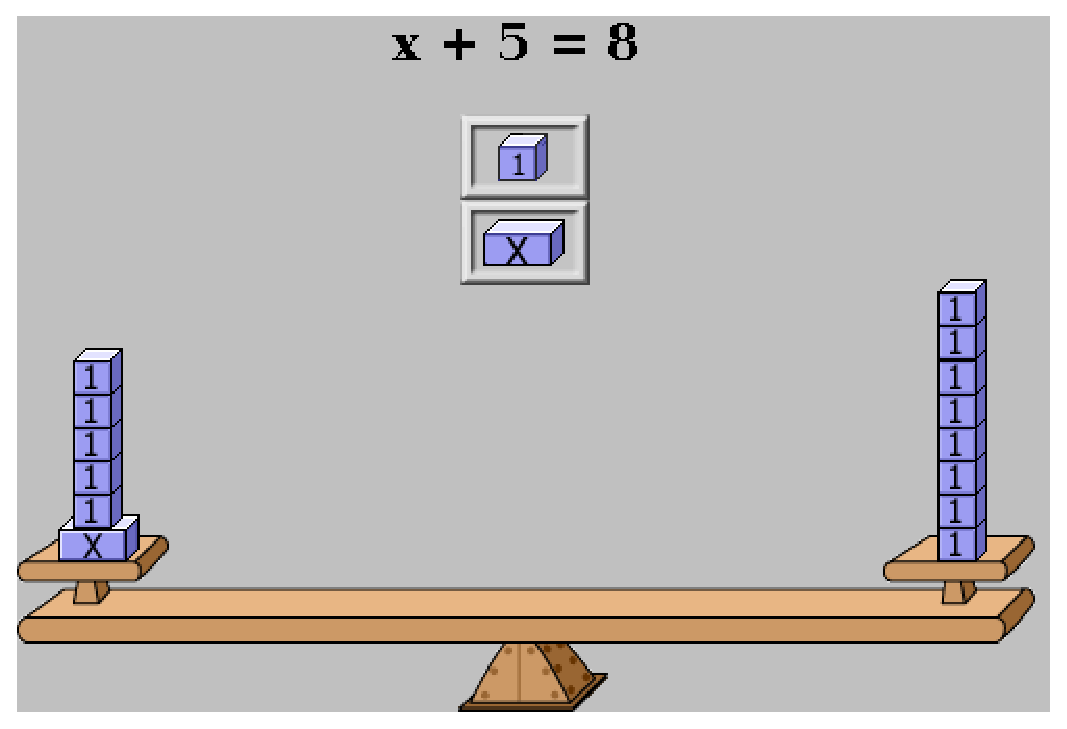
\includegraphics[width=5cm]{img/balanza}}{\scriptsize \par}

{\scriptsize{}\protect\caption{Ecuación Original}
}
\end{figure}
{\scriptsize \par}


\column{5cm}


\begin{center}
\textcolor{red}{\uline{Explicación }}
\par\end{center}


Inicialmente tenemos la ecuación ${\color{cyan}x+5=8}$ \\
{\small{}¿Qué pasa si quitamos 5 unidades de la derecha y de la izquierda?\pause{}}\\
{\small{}La balanza se debería mantener, puesto que quitamos las mismas
unidades. \pause{}}\\
{\small{}Algebraicamente: ${\color{cyan}x+5}{\color{red}-5}{\color{cyan}=8}{\color{red}-5}$
(hemos restado ambos miembros por 5)}{\small \par}

\end{columns}

\end{block}
\end{frame}

\begin{frame}{Reglas de equivalencia. Sumas y restas}

\begin{block}{}
{\scriptsize{}{x+5=8 (Continuación)}}{\scriptsize \par}
\begin{columns}[c]


\column{5cm}


\begin{center}
\textcolor{red}{\uline{Balanza Algebraica}}
\par\end{center}


{\scriptsize{}}
\begin{figure}
{\scriptsize{}\includegraphics[width=5cm]{img/balanza2}}{\scriptsize \par}

{\scriptsize{}\protect\caption{Ecuación Equivalente}
}
\end{figure}
{\scriptsize \par}


\column{5cm}


\begin{center}
\textcolor{red}{\uline{Explicación }}
\par\end{center}


Fíjate: Inicialmente teníamos la ecuación \textcolor{cyan}{$x+5=8$}
\\
{\small{}Hemos quitado 5 unidades a ambos miembros. La balanza se
mantiene en equilibrio. ¿Cuál es la ecuación equivalente resultante?\pause{}}\\
{\small{}${\color{cyan}x+5-5=8-5}$, que operando es:}\\
{\small{}${\color{cyan}x=3}$ \pause{}}\\
\textcolor{red}{\small{}Solución:}{\small{} \pause{}x vale 3.}{\small \par}

\end{columns}

\end{block}

\textcolor{red}{\emph{De manera práctica:}} El 5 está sumando en un
miembro, pasa al otro restando (y al revés uno restando pasa al otro
lado sumando)

\end{frame}

\begin{frame}{Ejercicios de Regla de equivalencia}

\begin{alertblock}{Recuerda: Regla de equivalencia de sumas y restas}

\begin{itemize}
\item Si sumamos o restamos la misma cantidad a ambos miembros de una ecuación
obtenemos otra ecuación equivalente a la primera
\item O de forma práctica, un término que está sumando puede pasar al otro
lado restando. O si está restando pasará sumando
\end{itemize}
\end{alertblock}

Resuelve las siguientes ecuaciones
\begin{columns}[t]


\column{3cm}


\begin{center}
$x+7=12$\pause{}
\par\end{center}


\begin{center}
\textcolor{blue}{$x+7-7=12-7$}
\par\end{center}


\begin{center}
\textcolor{blue}{$x=5$}
\par\end{center}


\begin{center}
Solución: x es 5\pause{}
\par\end{center}


\column{3cm}


\begin{center}
$5+x=12$\pause{}
\par\end{center}


\begin{center}
\textcolor{blue}{$5+x-5=12-5$}
\par\end{center}


\begin{center}
\textcolor{blue}{$x=7$}
\par\end{center}


\begin{center}
Solución: x es 7\pause{}
\par\end{center}


\column{3cm}


\begin{center}
$5=12+x$\pause{}
\par\end{center}


\begin{center}
\textcolor{blue}{$5-12=12+x-12$}
\par\end{center}


\begin{center}
\textcolor{blue}{$-7=x$}
\par\end{center}


\begin{center}
Solución: x es -7\pause{}
\par\end{center}

\end{columns}

\end{frame}

\begin{frame}{Reglas de equivalencia. Multiplicación y división}


Las ecuaciones podemos representarlas con una balanza:
\begin{block}{}
{\scriptsize{}{2x=6}}{\scriptsize \par}
\begin{columns}[c]


\column{5cm}


\begin{center}
\textcolor{red}{\uline{Balanza Algebraica}}
\par\end{center}


{\scriptsize{}}
\begin{figure}
{\scriptsize{}\includegraphics[width=5cm]{img/Balanza3}}{\scriptsize \par}

{\scriptsize{}\protect\caption{Ecuación Original}
}
\end{figure}
{\scriptsize \par}


\column{5cm}


\begin{center}
\textcolor{red}{\uline{Explicación }}
\par\end{center}


Inicialmente tenemos la ecuación ${\color{cyan}2x=6}$ \\
{\small{}¿Qué pasa si quitamos la mitad del peso de la derecha y de
la izquierda?\pause{}}\\
{\small{}La balanza se debería mantener, puesto que quitamos la mitad
de cada lado. \pause{}}\\
{\small{}Algebraicamente: ${\color{cyan}2x}{\color{red}:2}{\color{cyan}=6}{\color{red}:2}$
(hemos dividido ambos miembros por 2)}{\small \par}

\end{columns}

\end{block}
\end{frame}

\begin{frame}{Reglas de equivalencia. Multiplicación y división}

\begin{block}{}
{\scriptsize{}{2x=6 (Continuación)}}{\scriptsize \par}
\begin{columns}[c]


\column{5cm}


\begin{center}
\textcolor{red}{\uline{Balanza Algebraica}}
\par\end{center}


{\scriptsize{}}
\begin{figure}
{\scriptsize{}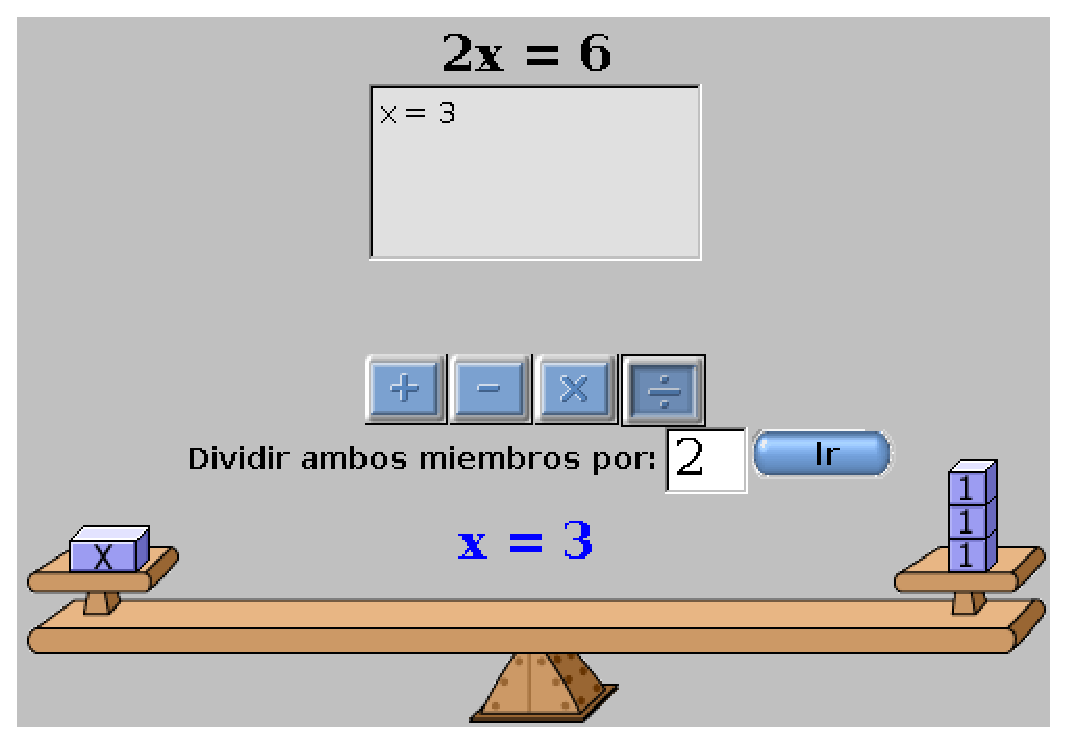
\includegraphics[width=5cm]{img/Balanza4}}{\scriptsize \par}

{\scriptsize{}\protect\caption{Ecuación Equivalente}
}
\end{figure}
{\scriptsize \par}


\column{5cm}


\begin{center}
\textcolor{red}{\uline{Explicación }}
\par\end{center}


Fíjate: Inicialmente teníamos la ecuación \textcolor{cyan}{$2x=6$}
\\
{\small{}Hemos quitado la mitad de unidades a ambos miembros. La balanza
se mantiene en equilibrio. ¿Cuál es la ecuación equivalente resultante?\pause{}}\\
{\small{}${\color{cyan}\frac{2x}{2}=\frac{6}{2}}$, que operando es:}\\
{\small{}${\color{cyan}x=3}$ \pause{}}\\
\textcolor{red}{\small{}Solución:}{\small{} \pause{}x vale 3.}{\small \par}

\end{columns}

\end{block}

\textcolor{red}{\emph{De manera práctica:}} El 2 está multiplicando
a la x, pasa al otro dividiendo a todo (y al revés algo dividiendo
pasa al otro lado multiplicando)

\end{frame}

\begin{frame}{Ejercicios de Regla de equivalencia}

\begin{alertblock}{Recuerda: Regla de equivalencia de multiplicación  y división}

\begin{itemize}
\item Si multiplicamos o dividimos la misma cantidad a ambos miembros de
una ecuación obtenemos otra ecuación equivalente a la primera
\item O de forma práctica, un número que está multiplicando a todo el miembro
puede pasar al otro lado dividiendo. O si está dividiendo pasará multiplicando
\end{itemize}
\end{alertblock}

Resuelve las siguientes ecuaciones
\begin{columns}[t]


\column{3cm}


\begin{center}
$3x=12$\pause{}
\par\end{center}


\begin{center}
\textcolor{blue}{$\frac{3x}{3}=\frac{12}{3}$}
\par\end{center}


\begin{center}
\textcolor{blue}{$x=4$}
\par\end{center}


\begin{center}
Solución: x es 4\pause{}
\par\end{center}


\column{3cm}


\begin{center}
$\frac{x}{5}=10$\pause{}
\par\end{center}


\begin{center}
\textcolor{blue}{$\frac{5x}{5}=10\cdot5$}
\par\end{center}


\begin{center}
\textcolor{blue}{$x=50$}
\par\end{center}


\begin{center}
Solución: x es 50\pause{}
\par\end{center}


\column{3cm}


\begin{center}
$24=12x$\pause{}
\par\end{center}


\begin{center}
\textcolor{blue}{$\frac{24}{12}=\frac{12x}{12}$}
\par\end{center}


\begin{center}
\textcolor{blue}{$2=x$}
\par\end{center}


\begin{center}
Solución: x es 2\pause{}
\par\end{center}

\end{columns}

\end{frame}

\subsection{Resolución general de ecuaciones}
\begin{frame}{Resolución general de ecuaciones}


Veamos como resolver ecuaciones más complejas, fíjate en los pasos:
\begin{columns}[c]


\column{7cm}
\begin{block}{7x-2=5x+4}

\begin{itemize}
\item Primero: {\footnotesize{}Realizamos una transposición de términos
pasando a un miembro todos los términos que contienen la incógnita
y al otro miembro los que no la contienen:}{\footnotesize \par}


\begin{center}
$7x{\color{red}-2}={\color{red}5x}+4$\pause{}
\par\end{center}


\begin{center}
${\color{cyan}7x-5x=4+2}$\pause{}
\par\end{center}

\item Segundo: {\footnotesize{}Realizamos las operaciones correspondientes:}\pause{}


\begin{center}
\textcolor{cyan}{$2x=6$}
\par\end{center}

\item Tercero: {\footnotesize{}Despejamos la incognita:}\pause{}


\begin{center}
\textcolor{cyan}{$x=\frac{6}{2}$}
\par\end{center}


\begin{center}
\textcolor{cyan}{$x=3$}
\par\end{center}

\end{itemize}
\end{block}

\column{3cm\pause{}}


{\small{}Es una buena costumbre comprobar la solución:}{\small \par}


\begin{center}
$7x-2=5x+4$ si hacemos x=3 \pause{}
\par\end{center}


\begin{center}
\textcolor{blue}{$7\cdot3-2=5\cdot3+4$}
\par\end{center}


\begin{center}
\textcolor{blue}{$21-2=15+4$}
\par\end{center}


\begin{center}
\textcolor{blue}{$19=19$}
\par\end{center}

\end{columns}

\end{frame}

\begin{frame}{Ejercicios}


Resuelve las siguientes ecuaciones
\begin{columns}[t]


\column{3cm}


\begin{center}
$3x-3=12$\pause{}
\par\end{center}


\begin{center}
\textcolor{blue}{$3x=12+3$}
\par\end{center}


\begin{center}
\textcolor{blue}{$3x=15$}
\par\end{center}


\begin{center}
\textcolor{blue}{$x=\frac{15}{3}$}
\par\end{center}


\begin{center}
\textcolor{blue}{$x=5$}
\par\end{center}


\begin{center}
Solución: x es 5\pause{}
\par\end{center}


\column{3cm}


\begin{center}
$\frac{x}{5}-3=12$\pause{}
\par\end{center}


\begin{center}
\textcolor{blue}{$\frac{x}{5}=12+3$}
\par\end{center}


\begin{center}
\textcolor{blue}{$\frac{x}{5}=15$}
\par\end{center}


\begin{center}
\textcolor{blue}{$x=15\cdot5$}
\par\end{center}


\begin{center}
\textcolor{blue}{$x=75$}
\par\end{center}


\begin{center}
Solución: x es 75\pause{}
\par\end{center}


\column{3cm}


\begin{center}
$24-3x=12x-21$\pause{}
\par\end{center}


\begin{center}
\textcolor{blue}{$24+21=12x+3x$}
\par\end{center}


\begin{center}
\textcolor{blue}{$45=15x$}
\par\end{center}


\begin{center}
\textcolor{blue}{$\frac{45}{15}=x$}
\par\end{center}


\begin{center}
\textcolor{blue}{$3=x$}
\par\end{center}


\begin{center}
Solución: x es 3\pause{}
\par\end{center}

\end{columns}

\end{frame}

\begin{frame}{Problemas con ecuaciones}


{\small{}Algunos }\textbf{\small{}problemas}{\small{} se pueden resolver
traduciendo el lenguaje natural a lenguaje algebraico, y en el caso
de obtener una ecuación y resolverla}{\small \par}
\begin{exampleblock}{Enunciado}El doble de un número menos 2 es 8. ¿Qué número es?\pause{}
\end{exampleblock}
\begin{columns}[c]


\column{5cm}
\begin{itemize}
\item No conocemos el número, luego le llamo x\pause{}
\item ``el doble de un número menos 2''\pause\rightarrowfill{}${\color{red}2x-2}$
\item ``es igual a 8'' \pause\rightarrowfill{}\textcolor{red}{$2x-2=8$}
\end{itemize}

\column{5cm}
\begin{itemize}
\begin{singlespace}
\item Resuelvo la ecuación:
\end{singlespace}

\begin{itemize}
\item \textcolor{blue}{$2x-2=8$}
\item \textcolor{blue}{$2x=10$}
\item \textcolor{blue}{$x=\frac{10}{2}$}
\item \textcolor{blue}{$x=5$}
\end{itemize}
\item Comprobamos la solución: \pause{}El doble de 5 es 10, \pause{}si
le quito 2 obtengo 8
\end{itemize}
\end{columns}

\end{frame}

\begin{frame}{Problemas con ecuaciones}

\begin{exampleblock}{Enunciado}En una clase hay 28 alumnos y el número de chicos es inferior
en 4 al número de chicas. ¿Cuántos chicos y chicas hay?\pause{}
\end{exampleblock}
\begin{columns}[c]


\column{5cm}
\begin{itemize}
\item No conocemos el número de chicos, luego le llamo x. Nota que cuando
resuelva la ecuación x será el número de chicos (no de chicas).\pause{}
\item ``el número de chicos es inferior en 4 al de chicas''. Chicas hay
\pause\rightarrowfill{}${\color{red}x+4}$
\item ``en total hay 28'' \pause\rightarrowfill{}\textcolor{red}{$x+\left(x+4\right)=28$}
\end{itemize}

\column{5cm}
\begin{itemize}
\begin{singlespace}
\item Resuelvo la ecuación:
\end{singlespace}

\begin{itemize}
\item \textcolor{blue}{$x+\left(x+4\right)=28$}
\item \textcolor{blue}{$2x+4=28$}
\item \textcolor{blue}{$2x=24$}
\item \textcolor{blue}{$x=12$ (12 chicos y 12+4 chicas)}
\end{itemize}
\item Comprobamos la solución: \pause{}número de chicos es 12, \pause{}
el de chicas será 12+4=16, y 16+12=28 en total\end{itemize}
\end{columns}

\end{frame}

\end{document}
